
\chapter{Lecture}\label{lec8}%%% 8

\setcounter{section}{3}
\section{Complements on \texorpdfstring{$H^m(\Omega)$}{Hm(Omega)}}\label{lec8:sec4} %sec 4

\subsection{Estimates on \texorpdfstring{$H^m_0(\Omega)$}{Hm0(Omega)}}\label{lec8:sec4:subsec1}

\begin{theorem}\label{lec8:sec4:subsec1:thm4.1}%thm 4.1
  Let\pageoriginale $\Omega$ be a bounded open set in $R^n$. Then there exists a $c
  >0$  such that $|u|_0\le c |u|_1$ for all $u \epsilon
  H^1_0(\Omega)$. 
\end{theorem}

\begin{proof}%proof
  Since $\mathscr{D}(\Omega)$ is dense in $H^1_o$ we need prove the
  inequality for $u = \varphi \epsilon \mathscr{D}$ $(\Omega)$. Let
  $\overset{\sim}{\varphi} = \varphi$ on $\Omega$ and $0$ outside
  $\Omega$ in $R^n$. 
  
  Since $\Omega$ is bounded, we have
  $$
  \overset{\sim}{\varphi}(x) = \int\limits_{-\infty}^{x_1}
  \frac{\partial}{\partial x_1} \varphi (t, x_2, \ldots , x_n) dt =
  \int\limits_{a}^{x_1} \frac{\partial \varphi }{\partial x_1} (t, x_2,
  \ldots , x_n) dt 
  $$
  where $a$ and $b$ are such that $\Omega$ is contained in the region
  determined by\break $]a, b[x R^{n-1}$. 
\end{proof}

By Schwartz's inequality
\begin{align*}
|\overset{\sim}{\varphi}(x)|^2  & \le (x_1 - a) \int\limits_a^b
|\frac{\partial \varphi}{\partial x_1}(t, x_2, \ldots , x_n)|^2 dt\\ 
& \le (b-a) \int\limits_a^b |\frac{\partial \varphi} {\partial x_1}
|(t, x_2, \ldots , x_n)|^2 dt. 
\end{align*}

Hence $\int |\overset{\sim}{\varphi}(x)|^2 dx \le (b-a)^2 \int_a^b
|\dfrac{\partial \varphi}{\partial x_1}|^2 dx$, and so $|\varphi|_0
\le (b-a) |\dfrac{\partial \varphi}{\partial x_1}|\le c |\varphi|_1$
as it was to be proved. 

\begin{remarks*}
~
\begin{enumerate}[(1)]
\item From the above proof it is seen that the theorem remains true
  even if $ \Omega$ is bounded only in any one direction. 
\item The theorem is not true for $H^1 (\Omega)$. Thus, for instance,
  if we take $u = 1$, then $u \epsilon H^1 (\Omega) $ and $|u|_0=$
  measure of and $|u|_1 = 0$, so there does not exists $c$ such that
  $|u|_0 \le c|u|_1$. 
\item The\pageoriginale theorem may remain true however for some spaces $V$ such that
  $H^1_o \subset V \subset H^1$. Thus if $\Omega$ is as shown in the
  figure and $V = u \epsilon H^1$ such that $u(0, x_2) = 0$, then
  $|u|_0 \le c |u|_1$. 
  \begin{figure}[H]
    \centering{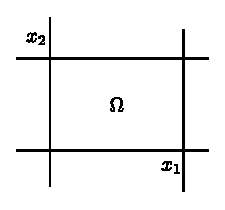
\includegraphics{vol10-figures/fig10-chap8-1.eps}}
  \end{figure}
\item If $u \in H^m_0 (\Omega)$, then $|u|_0 \le c|u|_m, |u|_k \le
  c|u|_m$, for $k \le m-1$. 
\end{enumerate}
\end{remarks*}

\noindent
\textbf{Applications: } We have already proved that for Dirichlet
problems $(V = H^1_0(\Omega))$ the operator $-\Delta + \lambda$
associated with the form $a(u, v) = (u, v)_1 + \lambda (u, v)_o$ is an
isomorphism of $H^1_o$ onto $H^{-1}_o$ for $\lambda > 0$. We now prove
the  
\begin{theorem}\label{lec8:sec4:subsec1:thm4.2}%thm 4.2
  If $\Omega$ is bounded, then $- \Delta + \lambda$ is an isomorphism of
  $H^1_o$ onto $H^{-1}_o$ for $\lambda > - \alpha$ for certain $\alpha >
  0$. 
\end{theorem}

\begin{proof}%proof
  We look for values of $\lambda$ for which $a(u, v)$ is $V$-elliptic,
  $$
  \text{i.e.,}\qquad \re a(u, u) = |u|^2_1 + \lambda |u|^2_0 \ge
  \gamma |u|^2_1.
  $$
  
 Since $\Omega$ is bounded $|u|^2_1 \ge \dfrac{1}{c^2} |u|^2_1$ for
 some $c > 0$, and  
 \begin{align*} 
   |u|^2_1 + \lambda |u|^2_0 & = |u|^2_1 + (\lambda - \epsilon
   )|u|^2_0 +\epsilon |u|^2_0\\ 
   & \ge (1 + (\lambda - \epsilon)c^2) |u|^2_1 + \epsilon |u|^2_0\\
   & \ge \gamma \| u \|^2_1 \text{ for positive } \gamma if 1+ (\lambda -
   \epsilon)c^2 > 0, 
 \end{align*}
 i.e., $\lambda > \dfrac{-1 + \epsilon c^2}{2}$. Choosing $\epsilon$
 sufficiently small, we have  $\alpha= \dfrac {1- c^2}{c^2}$ such
 that for $\lambda > 
 -\alpha, a(u, v)$ is V-elliptic and thus the theorem is proved.  
\end{proof}

\begin{theorem}\label{lec8:sec4:subsec1:thm4.3}%thm 4.3
  For every $\epsilon > 0$, there exists $c(\epsilon)$ such that
  $|u|^2_k \le \epsilon |u|^2_m + c(\epsilon) |u|^2_0$ for all $u
  \epsilon H^m_0(\Omega)$ and 0) $\le k \le m-1$.  
\end{theorem}

\begin{proof}%proof
  Let\pageoriginale $\overset{\sim}{u}$ be the function defined in $R^n$ which is
  equal to $u$ on $\Omega$ an $0$ elsewhere. We have then
  $|\overset{\sim}{u}|_m = |u|_m$. Let $\overset{\sim}{u} = \mathscr{F}
  (\overset{\sim}{u})$ be the Fourier transform of
  $\overset{\sim}{u}$. By Plancherel's theorem  
  $$
  |\overset{\sim}{u}|^2_k = \sum\limits_{p = k} (2  \pi)^{2k} \int
  \limits_{\mathbb{Z}^n} |\xi|^{2k} |\overset{\sim}{u}|^2 d \xi =
  |\overset{\sim}{u}|^2_k = |u|^2_k. 
  $$
  
  To verify the stated inequality it is enough to prove that for
  $\epsilon > 0$ there exists $c(\epsilon)$ such that 
  \begin{gather*}
    (2\pi)^{2k}\int |\xi|^{2k}|\hat{u}|^2 d \xi \le (2\pi)^{2m}
    \epsilon \int |\xi|^{2m}|\hat{u}|^2 d \xi + c(\epsilon)
    \int |\hat{u}|^2 d \xi, \\
    \text{i.e.,}\qquad \int |\xi|^{2k} |\hat{u}|^2 d \xi \le \int
    (\epsilon(2\pi)^{2m-2k}|\xi|^{2m}+
    \frac{c(\epsilon)}{(2\pi)^{2k}}) |\hat{u}|^2 d\xi.
  \end{gather*}
  
  This will be true if 
  $$
  |\xi|^{2k} \le \epsilon_1 |\xi|^{2m} + c_1 (\epsilon) \quad for
  \quad k \le m-1. 
  $$
  
  Since $k \le m-1$, for any $\epsilon_1 > 0, |\xi|^{2k} \le
  \epsilon_1 |\xi|^{2m}$ for large values of $\xi$ and for remaining
  necessarily bounded values of $\xi, |\xi|^{2k} - \epsilon_1
  |\xi|^{2m}$ is bounded by $C_1 (\epsilon)$ say. 
\end{proof}

\begin{remark*}%Remark
  The status of this theorem is different from that of the theorem
  $4.1$: for it may be sometime true for $H^m(\Omega)$ also. As we shall
  see later, this is connected with the problem of m-regularity. For
  example, if $\Omega = ]0, 1[$, theorem \ref{lec8:sec4:subsec1:thm4.3} holds for $u \epsilon
  H^m(\Omega)$. 
\end{remark*}

\subsection{Regularity of the function in \texorpdfstring{$H^m(\Omega)$}{Hm(Omega)}}\label{lec8:sec4:subsec2}%sec 2 

\begin{theorem}\label{lec8:sec4:subsec2:thm4.4}%thm 4.4
 If $2m >n, H^m (\Omega) \subset \mathscr{E}^o (\Omega)$ algebraically
 and topologically. 
\end{theorem}

\begin{proof}
Let $u \epsilon H^m(\Omega)$. We need prove that for every $\varphi
\epsilon \mathscr{D} (\Omega), v = u \varphi \epsilon
\mathscr{E}^o (\Omega)$. Since $v$ vanishes near the boundary of
$\Omega$, the function $\tilde{v}$ is in $H^m_o(R^n)$. Let
$\tilde{v}$  be the Fourier transform of $\tilde{v}$, 
\end{proof}
then\pageoriginale $(1 + |\xi |^m) \hat{v} \epsilon L^2$. Now,
$$
\hat{v} = (1+ |\xi|^m) \hat{v}. \frac{1}{1 + |\xi|^m}.
$$

Since $2m > n$,
$$
\int\limits_{\mathbb{Z}} |\frac{1}{1 + |\xi|^m}|^2 d \xi = O
(\int\limits_{o}^{\infty} \frac{r^{n-1}}{1+ r^n} dr)< \infty. 
$$

Hence $\hat{u} \epsilon L^1$. That is to say $v$ is continuous.

If now $u \to 0$ in $H' (\Omega)$ we have $\hat{v} \to 0$ in $L^1$.

Hence $v \to 0$ in $\xi^o (\Omega)$ and so $u \to 0$ in $\xi^o$

\begin{remark*}
  Better results valid for more general classes of domains are due to
  Soboleff. A typical result is if $n \geq 3$, then $u \epsilon H'
  (\Omega) \Longrightarrow u \in L^q (\Omega) , \dfrac{1}{q} = \dfrac{1}{2}-
  \dfrac{1}{n}$, for certain $\Omega$. (viz., Deny-Lions \cite{k7} and also
  Schwartz [\ref{k16:e1}]). 
\end{remark*}

\subsection{Reproducing kernels}\label{lec8:sec4:subsec3}

Let $v$ be a closed subspace of $H^m (\Omega)$ such that $H^m_o
(\Omega) \subset V \subset H^m (\Omega)$ and $Q = L^2 (\Omega)$. Let
$a (u , v)$ be a continuous sesquilinear from on $V$. Assume now
\textit{$2m > n$}. Hence in each class of functions $v \epsilon V$,
there exists a \textit{unique} continuous function $v_o $(say). Then,
for fixed $y \epsilon \Omega$, the mapping $v \to \overline{v_o
  (y)}$ is a continuous semilinear form on $V$. Hence by Riesz's
theorem, there exists $k (y) \epsilon V$ such that $\overline{v_o
  (y)} = (k (y) , v)_V$. The mapping $y \to k(y)$ is weakly continuous
mapping of $\Omega$ into $V$. 

\begin{definition}\label{lec8:sec4:subsec3:def4.1}%def 4.1
  $k(y)$ is called reproducing kernel in $V$ (Aronszajn [\ref{k2:e2}]). 
\end{definition}

If $a(u,v)$ is V-elliptic we have by theorem \ref{lec5:sec3:subsec2:thm3.1}

\begin{lemma}\label{lec8:sec4:subsec3:lem4.1}%lem 4.1
  For every $y \epsilon \Omega$ there exists unique $g (y)
  \epsilon V$ such that $a (g (y), v) = (k (y), v )_V$ and the
  mapping $y \to g(y)$ of $\Omega \to V$ is weakly continuous.  
\end{lemma}

We\pageoriginale now relate the $V$ valued function $g(y)$ with the Green's operator
$a(u,v)$ in $V$. For every $v \epsilon V$, we have  
$$
a(g (y),v) = \overline{v(y)}.
$$

Hence, for any $\varphi \epsilon \mathscr{D} (\Omega), a (\varphi
(y) g(y), v) = \varphi (y) \overline{v(y)}$. 

Integrating over $\Omega, \int\limits_{\Omega} a (\varphi (y) g(y), v)
= (\varphi, v)_o$. Hence  
$$
a \left(\int\limits_{\Omega} g(y) \varphi (y) dy, v\right)= (\varphi , v)_o
$$
where $\int\limits_{\Omega} g(y) \varphi(y)$ by is a weak
integral. Now since $a(u,v)$ is $V$-elliptic, given $\varphi
\epsilon \mathscr{D} (\Omega)$, there exists $u \epsilon V$ such
that $Au = \varphi$, $a (u,v) = (\varphi, v)_o$ for all $v \epsilon
V$, and $u = G \varphi$. Hence 
$$
G \varphi = u = \int\limits_{\Omega}g(y) \varphi (y) dy.
$$
\begin{theorem}\label{lec8:sec4:subsec3:thm4.5}%the4.5
  Let $\Omega$ be an open set in $R^n$ and  $2m > n$. Let $V, Q,
  a(u,v)$ be as above. Then $G \varphi = \int\limits_{\Omega} g(y)
  \varphi (y) ~dy$ where $g(y) V$, and is given by $a (g (y), v)=
  \overline{v(y)}$. 
\end{theorem}

This is a particular case of Schwartz's kernel theorem.

The kernel $G_{x,y}$ defined by the operator $G$ in \ref{lec7:sec3:subsec4:thm3.5} is $g(y) (x)$. 

There is yet another way of defining the $V$-valued function $g(y)$. Let
$Q = L^2 (\Omega) \cap \varepsilon^o (\Omega)$. On $Q$ we put the upper bound
topology of $L^2$ and $\varepsilon^o$. Since $2m >n$ any $V$ such that $H^m_o
(\Omega) \subset V \subset H^m (\Omega)$ is contained in $\varepsilon^o
(\Omega)$, and hence in $Q$. Further since $\mathscr{D} (\Omega)$ is
hence in $Q$. If $a (u , v)$ is a continuous sesquilinear $V$-elliptic
from on $V$, from theorem \ref{lec5:sec3:subsec2:thm3.1} it follows that there exists a space $N
\subset V$ and an operator $A$, such that $A$ is an isomorphism of $N$
onto $Q'$. 

Now\pageoriginale
\begin{align*}
  Q' & = (L^2 (\Omega))' + (\varepsilon^o (\Omega))\\
  & = L^2 (\Omega ) + \varepsilon'^o (\Omega)
\end{align*}
where $\varepsilon'^o (\Omega)$ is the space of measures with compact support. 

Let $G$ be the inverse operators of $A; G$ is an isomorphism of $Q'$
onto $N$. Then $g(y) = G (\delta_y)$. 

\begin{remark*}
  $G$ as defined here, has slightly different meaning from the one
  defined previously, but the abuse of language is justified since
  both of these are inverse of the restriction of the same operator
  $\mathscr{A}: V \to \mathscr{D}'$, see \S\ \ref{lec7:sec3:subsec4}. 
\end{remark*}
